\documentclass[]{article}
\usepackage{geometry,tikz,lipsum,amsmath,amssymb,soul,cancel,esint,eso-pic}
\usepackage[dvipsnames]{xcolor}

\definecolor{verde}{rgb}{0.844, 1.000, 0.753}
\definecolor{azul}{rgb}{ 0.858, 0.930, 1.000}
\definecolor{rojo}{rgb}{ 1.000, 0.788, 0.730}

\tikzset{every picture/.style={line width=0.75pt}} %set default line width to 0.75pt
\usetikzlibrary{tikzmark,fit}

\numberwithin{equation}{section}

\NewDocumentCommand{\caja}{ m O{gray!40} O{gray!10} m }{
	\begin{figure}[h]
		\centering
		\begin{tikzpicture}
			\node[anchor=text, text width=\columnwidth-1.2cm, draw, rounded corners, line width=1pt, fill=#3, inner sep=5mm] (big) {\\#4};
			\node[draw, rounded corners, line width=.5pt, fill=#2, anchor=west, xshift=5mm] (small) at (big.north west) {#1};
		\end{tikzpicture}
	\end{figure}
}
\NewDocumentCommand{\indUpDown}{ O{\Lambda} O{\mu} O{\nu} }{
	{#1}^{#2}_{\ #3}
}
\NewDocumentCommand{\indDownUp}{ O{\Lambda} O{\mu} O{\nu} }{
	{#1}_{#2}^{\ #3}
}
\newcommand{\LambdaMuNu}{\indUpDown}
\newcommand{\0}{\textcolor{gray}{0}}
\newcommand{\ei}{\mathbf{e}_i}
\newcommand{\ej}{\mathbf{e}_j}
\newcommand{\lc}{\epsilon_{ijk}}
\newcommand{\gr}{\nabla}
\newcommand{\di}{\nabla\cdot}
\newcommand{\ro}{\nabla\times}
\newcommand{\la}{\nabla^2}
\newcommand{\rv}{\mathbf{r}}
\newcommand{\xv}{\mathbf{x}}
\newcommand{\yv}{\mathbf{y}}
\newcommand{\zv}{\mathbf{z}}
\newcommand{\xhat}{\hat{\xv}}
\newcommand{\yhat}{\hat{\yv}}
\newcommand{\zhat}{\hat{\zv}}
\newcommand{\ihat}{\hat{\mathbf{i}}}
\newcommand{\jhat}{\hat{\mathbf{j}}}
\newcommand{\khat}{\hat{\mathbf{k}}}
\newcommand{\rhat}{\hat{\rv}}
\newcommand{\that}{\hat{\mathbf{\theta}}}
\newcommand{\phat}{\hat{\mathbf{\varphi}}}
\newcommand{\rhhat}{\hat{\mathbf{\rho}}}
\newcommand{\nhat}{\hat{\mathbf{n}}}
\newcommand{\Rhat}{\hat{\mathbf{R}}}
\newcommand{\eo}{\epsilon_{0}}
\newcommand{\uo}{\mu_{0}}
\NewDocumentCommand{\ke}{ O{1}}{
	\frac{#1}{4\pi\eo}
}
\NewDocumentCommand{\ku}{ O{}}{
	\frac{\uo #1}{4\pi}
}
%\newcommand{\ke}{\frac{1}{4\pi\eo}}
%\newcommand{\ku}{\frac{\uo}{4\pi}}
\newcommand{\rdif}{\rv - \rv'}
\newcommand{\pd}[2]{\dfrac{\partial #1}{\partial #2}}
\newcommand{\lpd}[2]{\partial #1/\partial #2}
\newcommand{\td}[2]{\dfrac{d #1}{d #2}}
\newcommand{\ltd}[2]{d #1/d #2}
\newcommand{\n}[1]{\mathbf{#1}}
\newcommand{\eff}[1]{#1_\mathrm{eff}}
\newcommand{\Ueff}{\eff{U}}

\newcommand{\wfrac}[3][3pt]{%
	\frac{\wfracterm{depth}{\dp}{#1}{#2}}{\wfracterm{height}{\ht}{#1}{#3}}%
}
\newcommand{\wfracterm}[4]{%
	\sbox0{$\displaystyle#4$}%
	\vrule width 0pt #1 \dimexpr #20+#3\relax
	\usebox{0}%
}

%opening
\title{Tarea 3 Mecánica Clásica Avanzada}
\author{Simon Fonseca}

\begin{document}
\maketitle
\section{Pregunta 1}
A relativistic particle of mass \(m\) interacts with an external symmetric rank-2 tensor field \(S^{\mu\nu}\), so the action is given by
\begin{equation}
	S = \int \Lambda \, d\tau, ~~~~~~~ \Lambda = -mc^2 \sqrt{\dot{x}_\mu \dot{x}^\mu} + e \dot{x}_\mu \dot{x}_\nu S^{\mu\nu}(x) \label{enunciado}
\end{equation}
where \(\tau\) is the proper time, \(x^\mu\) is the trajectory of the particle, and \(\dot{x}^\mu = \ltd{x^\mu}{\tau} \equiv u^\mu\) is the 4-velocity of the particle.

\begin{enumerate}
	\item[\textbf{a.}] Write out the generalized momentum \(P_\mu = \lpd{\Lambda}{\dot{x}^\mu}\) and the equations of motion in covariant form which correspond to the lagrangian.
	
	Escribiendo el lagrangiano covariante en términos de \(\dot{x}^{\mu}\), y cambiando los índices \textit{dummy},
	\begin{equation}
		\Lambda = -mc^2 \sqrt{\eta_{\alpha\rho} \dot{x}^\alpha \dot{x}^\rho} + e \, \eta_{\beta\rho} \dot{x}^\beta \, \eta_{\lambda\sigma} \dot{x}^\lambda \, S^{\rho\sigma}(x)
	\end{equation}
	Tenemos
	\begin{align}
		P_\mu = \pd{\Lambda}{\dot{x}^\mu} &= \pd{}{\dot{x}^\mu} \left(-mc^2 \sqrt{\eta_{\alpha\rho} \dot{x}^\alpha \dot{x}^\rho} + e \, \eta_{\beta\rho} \dot{x}^\beta \, \eta_{\lambda\sigma} \dot{x}^\lambda \, S^{\rho\sigma}(x) \right) \nonumber\\
		&= -mc^2 \frac{1}{2 \sqrt{\eta_{\alpha\rho} \dot{x}^\alpha \dot{x}^\rho}} \pd{}{\dot{x}^\mu} \left( \eta_{\alpha\rho} \dot{x}^\alpha \dot{x}^\rho \right) + e S^{\rho\sigma} \eta_{\beta\rho} \eta_{\lambda\sigma} \pd{}{\dot{x}^\mu} \left( \dot{x}^\beta \dot{x}^\lambda \right) \nonumber\\
		&= -mc^2 \frac{1}{2 \sqrt{\eta_{\alpha\rho} \dot{x}^\alpha \dot{x}^\rho}} \left( \eta_{\alpha\rho} \delta^\alpha_\mu \dot{x}^\rho + \eta_{\alpha\rho} \dot{x}^\alpha \delta^\rho_\mu \right) + e S^{\rho\sigma} \eta_{\beta\rho} \eta_{\lambda\sigma} \left( \delta^\beta_\mu \dot{x}^\lambda + \dot{x}^\beta \delta^\lambda_\mu \right) \nonumber\\
		&= -mc^2 \frac{1}{2 \sqrt{\dot{x}^\alpha \dot{x}_\alpha}} \left( \eta_{\mu\rho} \dot{x}^\rho + \eta_{\alpha\mu} \dot{x}^\alpha \right) + e \left( \eta_{\mu\rho} \eta_{\lambda\sigma} S^{\rho\sigma} \dot{x}^\lambda + \eta_{\beta\rho} \eta_{\mu\sigma} S^{\rho\sigma} \dot{x}^\beta \right)\nonumber
		\intertext{Como \(S\) es un tensor,}
		&= -mc^2 \frac{1}{2 \sqrt{\dot{x}^\alpha \dot{x}_\alpha}} \left( \dot{x}_\mu + \dot{x}_\mu \right) + e \left( \eta_{\mu\rho}  S^{\rho}_{\, \lambda} \dot{x}^\lambda + \eta_{\beta\rho} S^{\rho}_{\, \mu} \dot{x}^\beta \right) \nonumber\\
		&= -mc^2 \frac{\dot{x}_\mu}{\sqrt{\dot{x}^\alpha \dot{x}_\alpha}} + e \left(S_{\mu\lambda} \dot{x}^\lambda + S_{\beta\mu} \dot{x}^\beta \right) \nonumber
		\intertext{En el primer término, \(\alpha\) es un índice mudo, por lo que podemos cambiarlo a \(\mu\) por conveniencia. En el segundo término, los índices \(\lambda, \beta\) son mudos en sus respectivas sumatorias, por lo que podemos cambiarlos a \(\nu\),}
		&= -mc^2 \frac{\dot{x}_\mu}{\sqrt{\dot{x}^\mu \dot{x}_\mu}} + e \left(S_{\mu\nu} \dot{x}^\nu + S_{\nu\mu} \dot{x}^\nu \right)\nonumber
		\intertext{Pero \(S\) es un tensor simétrico, por lo que \(S_{\nu\mu} = S_{\mu\nu}\). En unidades naturales, \(c = 1\):}
		P_\mu = \pd{\Lambda}{\dot{x}^\mu} &= -m \frac{\dot{x}_\mu}{\sqrt{\dot{x}^\mu \dot{x}_\mu}} + 2 \, e \, \dot{x}^\nu S_{\mu\nu}
	\end{align}
	Finalmente, las ecuaciones de movimiento,
	\begin{equation*}
		\td{P_\mu}{\tau} = \pd{\Lambda}{x^\mu}
	\end{equation*}
	Del lado izquierdo tendremos
	\begin{align*}
		\td{P_\mu}{\tau} &= -m \frac{\ddot{x}_\mu}{\sqrt{\dot{x}^\mu \dot{x}_\mu}} - m \dot{x}_\mu \td{}{\tau}\left(\dot{x}^\mu \dot{x}_\mu\right)^{-1/2} + 2 \, e \, \ddot{x}^\nu S_{\mu\nu} + 2 \, e \, \dot{x}^\nu \td{S_{\mu\nu}}{\tau}
		\intertext{Reemplazando \(\dot{x}^\mu \dot{x}_\mu = u^\mu u_\mu = 1\),}
		&= -m \ddot{x}_\mu - 0 + 2 \, e \, \ddot{x}^\nu S_{\mu\nu} + 2 \, e \, \dot{x}^\nu \td{x^\alpha}{\tau} \pd{S_{\mu\nu}}{x^\alpha}\\
		&= -m \ddot{x}_\mu + 2 \, e \, \ddot{x}^\nu S_{\mu\nu} + 2 \, e \, \dot{x}^\nu \dot{x}^\alpha \pd{S_{\mu\nu}}{x^\alpha}
	\end{align*}
	Y del lado derecho,
	\begin{align*}
		\pd{\Lambda}{x^\mu} &= -m \pd{}{x^\mu} \sqrt{\dot{x}_\mu \dot{x}^\mu} + \pd{}{x^\mu} e \, \dot{x}_\beta \dot{x}_\nu S^{\beta\nu}(x)\\
		&= 0 + e \, \dot{x}_\beta \dot{x}_\nu \pd{S^{\beta\nu}}{x^\mu}\\
		&= e \, \dot{x}^\beta \dot{x}^\nu \pd{S_{\beta\nu}}{x^\mu}
	\end{align*}
	Por lo que las ecuaciones de movimiento covariantes,
	\begin{equation*}
		-m \ddot{x}_\mu + 2 \, e \, \ddot{x}^\nu S_{\mu\nu} + 2 \, e \, \dot{x}^\nu \dot{x}^\alpha \pd{S_{\mu\nu}}{x^\alpha} = e \, \dot{x}^\beta \dot{x}^\nu \pd{S_{\beta\nu}}{x^\mu}
	\end{equation*}
	\begin{equation}
		\Rightarrow -m \ddot{x}_\mu + 2 \, e \, \ddot{x}^\nu S_{\mu\nu} + e \left(2 \dot{x}^\nu \dot{x}^\alpha \pd{S_{\mu\nu}}{x^\alpha} - \dot{x}^\beta \dot{x}^\nu \pd{S_{\beta\nu}}{x^\mu}\right) = 0
	\end{equation}
	
	\item[\textbf{b.}] Write out the non-covariant lagrangian \(L\) which corresponds to the lagrangian \ref{enunciado}. Simplify your result in the nonrelativistic limit.
	
	Para pasar a un lagrangiano no covariante podemos usar que
	\begin{equation}
		S = \int \Lambda \, d\tau = \int L \, dt
	\end{equation}
	Tomando \(c = 1\) y \(t = \gamma \, \tau\),
	\begin{align}
		L &= \frac{1}{\gamma} \Lambda\\
		&= \frac{1}{\gamma} \left(-mc^2 \sqrt{\dot{x}_\mu \dot{x}^\mu} + e \dot{x}_\mu \dot{x}_\nu S^{\mu\nu}(x)\right)\nonumber
	\end{align}
	Sabiendo que
	\begin{equation*}
		\dot{x}^\mu = \td{x^\mu}{\tau} = \td{t}{\tau} \td{x^\mu}{t} = \gamma \, v^\mu
	\end{equation*}
	tendremos
	\begin{align*}
		L &= \frac{1}{\gamma} \left(- \gamma mc^2 \sqrt{v_\mu v^\mu} + e \gamma^2 v_\mu v_\nu S^{\mu\nu}(x)\right) \\
		&= - mc^2 \sqrt{v_\mu v^\mu} + e \gamma v_\mu v_\nu S^{\mu\nu}(x)
	\end{align*}
	Ya que \(x^\mu = (t,\n{x})\) entonces \(v^\mu = (1, \n{v})\) y \(v_\mu = (1, -\n{v})\), por lo que
	\begin{equation*}
		v_\mu v^\mu = 1 - |\n{v}|^2 = \frac{1}{\gamma^2}
	\end{equation*}
	entonces
	\begin{align*}
		L &= - \frac{1}{\gamma}mc^2 + e \gamma v_\mu v_\nu S^{\mu\nu}(x)
	\end{align*}
	En el caso del segundo término, tendremos que separar los casos \(\mu = 0, \nu = 0\) del resto para expresar el lagrangiano en términos espaciales:
	
	\begin{align}
		L &= - \frac{1}{\gamma}mc^2 + e \gamma \left(v_0 v_0 S^{00} + v_0 v_j S^{0j} + v_i v_0 S^{i0} + v_i v_j S^{ij}\right) \nonumber\\
		&= - \frac{1}{\gamma}mc^2 + e \gamma \left(S^{00} + 2 v_i S^{0i} + v_i v_j S^{ij}\right) \nonumber\\
		&= - \frac{1}{\gamma}mc^2 + e \gamma \left(S^{00} + 2 v_i S^{0i} + v_i v_j S^{ij}\right) \nonumber\\
		&= - \frac{1}{\gamma}mc^2 + e \gamma \left(S^{00} - 2 v^i S^{0i} + v^i v^j S^{ij}\right) \nonumber
		\intertext{Si definimos el escalar \(s(x) = S^{00}\), el vector \(\n{s}(x) = S^{0i}\), y escribimos la parte espacial de \(S^{\mu\nu}\) como una matriz \(3\times 3\), tal que \(\n{S} = S^{ij}\). Tendremos, en unidades naturales,}
		L &= - m \sqrt{1 - |\n{v}|^2} + \frac{e}{\sqrt{1 - |\n{v}|^2}} \left(s(x) - 2 \n{s}\cdot\n{v} + \n{v} \cdot \left(\n{S} \n{v}\right) \right)
	\end{align}
	
	Tomando el límite no relativista \(v \rightarrow 0\) (calculado con \texttt{Mathematica}),
	\begin{equation}
		L \approx - m + \frac{1}{2} m v^2 + e \left[\left(1 + \frac{1}{2} v^2 \right) s(x) - 2\n{s}\cdot\n{v} + \n{v} \cdot \left(\n{S} \n{v}\right)\right]
	\end{equation}
	
	\item[\textbf{c.}] Assume that in the laboratory reference frame the tensor \(S_{\mu\nu}\) in spherical coordinates is given by
	\begin{equation*}
		S_{\mu\nu}^{\mathrm{(sph)}} = \mathrm{diag} \, (S_{tt}, S_{rr}, S_{\theta\theta}, S_{\phi\phi}) = \mathrm{diag} \left(- \frac{a}{r}, - \frac{a}{r - a}, 0, 0\right)
	\end{equation*}
	where \(a\) is some constant, and the particle always moves in the region \(r \gg a\).
	\begin{enumerate}
		\item[i.] Identify all the continuous global symmetries of the action and construct the integrals of motion which may exist according to Noether's theorem.
		
		
		Ya que estamos usando una métrica plana, \(S_{\mu\nu} = \eta_{\mu\alpha} \eta_{\nu\beta} S^{\alpha\beta} = S^{\mu\nu}\). Además, la velocidad será:
		\begin{equation*}
			\n{v} = \dot{\rv} = \left(\dot{r}, ~r\dot{\theta}, ~r\dot{\phi}\sin\theta\right)
		\end{equation*}
		Tomando el lagrangiano no covariante y reemplazando los valores de \(S\):
		\AddToShipoutPictureBG*{%
			\begin{tikzpicture}[overlay,remember picture,opacity=1,inner sep=4pt]
				\node[fill=azul, fit=(m1.center)(m3.center)]{};
				\node[fill=verde,fit=(m7.west)(m8.center)]{};
				\node[fill=rojo, fit=(m2.west)(m4.center)]{};
				\node[fill=rojo, fit=(m5.west)(m6.east)]{};
			\end{tikzpicture}
		}
		\begin{equation}
			S = \begin{bmatrix}
				\textcolor{blue}{(s)} & \textcolor{Red}{\begin{pmatrix}
					\phantom{.} & \n{s} & \phantom{.}
				\end{pmatrix}} \\
				\textcolor{Red}{\begin{pmatrix}
					\phantom{.} \\
					\n{s} \\
					\phantom{.}
				\end{pmatrix}} & \textcolor{Green}{\begin{pmatrix}
				& & \\
				& \n{S} & \\
				\phantom{.}
				\end{pmatrix}}
			\end{bmatrix} = \begin{bmatrix}
				\tikzmarknode{m1}{-a} \tikzmarknode{m3}{/r} & \tikzmarknode{m2}{\hspace{7.5mm} 0 \hspace{7.5mm}} & 0 & \tikzmarknode{m4}{0} \\
				\tikzmarknode{m5}{0} & \tikzmarknode{m7}{-a/(r-a)} & 0 & 0 \\
				0 & 0 & 0 & 0 \\
				\tikzmarknode{m6}{0} & 0 & 0 & \tikzmarknode{m8}{0}
			\end{bmatrix}
		\end{equation}
		
		\begin{align}
			L &= - m \sqrt{1 - |\n{v}|^2} + \frac{e}{\sqrt{1 - |\n{v}|^2}} \left(s(x) - 2 \n{s}\cdot\n{v} + \n{v} \cdot \left(\n{S} \n{v}\right) \right) \nonumber\\
			&= - m \sqrt{1 - v^2} + \frac{e}{\sqrt{1 - v^2}} \left(-\frac{a}{r} - 0 - \frac{a}{r - a}\dot{r}^2\right)\nonumber\\
			&= - m \sqrt{1 - v^2} - \frac{e}{\sqrt{1 - v^2}} \left(\frac{a}{r} + \frac{a}{r - a}\dot{r}^2\right)\nonumber\\
			&= - \frac{1}{\gamma} m - \gamma \underbrace{e \left(\frac{a}{r} + \frac{a}{r - a}\dot{r}^2\right)}_{U(r,\dot{r})}
		\end{align}
		Ya que todos los términos dependen de \(r\) o \(\dot{r}\), podemos concluir que el sistema tiene simetría esférica. Explícitamente:
		\begin{equation}
			L = - m \sqrt{1 - \left(\dot{r}^2 + r^2\dot{\theta}^2 + r^2 \dot{\phi}^2 \sin^2\theta \right)} - \frac{e \left(\dfrac{a}{r} + \dfrac{a}{r - a}\dot{r}^2\right)}{\sqrt{1 - \left(\dot{r}^2 + r^2\dot{\theta}^2 + r^2 \dot{\phi}^2 \sin^2\theta \right)}}
		\end{equation}
		
		De la expresión del lagrangiano encontramos que \(t\) no aparece, por lo que \textbf{la energía se conserva}. Utilizando \texttt{Mathematica} y simplificando:
		\begin{align}
			E &= \sum_i \dot{q}_i \pd{L}{\dot{q}_i} - L \nonumber\\
			&= \frac{m}{\sqrt{1 - v^2}} + \frac{e}{\left(1 - v^2\right)^{3/2}} \left(\frac{a}{r} \left(1 - 2 v^2\right) - \frac{a}{r - a} \dot{r}^2 \right)\nonumber\\
			&= \left[m \gamma - e \gamma^3 \left(\dfrac{a}{r} + \dfrac{a}{r - a}\dot{r}^2\right)\right] + 2 e \gamma \frac{a}{r}
		\end{align}
		(en el último paso, la energía se dejó convenientemente escrita para lo que vendrá más tarde).
		
		Además, \(\phi\) es cíclica, por lo que se conservará el momento. Utilizando \texttt{Mathematica} y simplificando:
		\begin{align}
			M_z = p_\phi = \pd{L}{\dot{\phi}} &= \left[\frac{m}{\sqrt{1 - v^2}} - \frac{e}{\left(1 - v^2\right)^{3/2}} \left(\dfrac{a}{r} + \dfrac{a}{r - a}\dot{r}^2\right) \right] r^2 \dot{\phi} \sin^2\theta\nonumber\\
			&= \left[m \gamma - e \gamma^3 \left(\dfrac{a}{r} + \dfrac{a}{r - a}\dot{r}^2\right) \right] r^2 \dot{\phi} \sin^2\theta \label{Mz}
		\end{align}
		Pero, ya que el lagrangiano del sistema es esféricamente simétrico en las 3 dimensiones del espacio, el teorema de Noether nos dice se conservarán las 3 componentes del momento angular por separado, es decir:
		
		\begin{align}
			\n{M} = \n{r} \times \n{p} &= \n{r} \times \pd{L}{\n{v}}\nonumber\\
			&= \rv \times \pd{}{\n{v}} \left[ - m \sqrt{1 - |\n{v}|^2} - \frac{e}{\sqrt{1 - |\n{v}|^2}} \left(\frac{a}{r} + \frac{a}{r - a}\dot{r}^2\right) \right]\nonumber\\
			&= \rv \times \pd{}{\n{v}} \left[ - m \sqrt{1 - \n{v}\cdot\n{v}} - \frac{e}{\sqrt{1 - \n{v}\cdot\n{v}}} \left(\frac{a}{r} + \frac{a}{r - a}(\rhat\cdot\n{v})^2\right) \right]\nonumber\\
			&= \rv \times  \left[ \left( m\gamma - e\gamma^3 \left(\frac{a}{r} + \frac{a}{r - a}\dot{r}^2\right) \right) \n{v} - \left( \frac{2ea\gamma(\rv\cdot\n{v})}{r^2(r-a)} \right) \rv \right]\nonumber\\
			&= \left[ m\gamma - e\gamma^3 \left(\frac{a}{r} + \frac{a}{r - a}\dot{r}^2\right) \right] (\rv \times \n{v}) = \mathrm{const}
		\end{align}
		Al analizar este resultado en coordenadas cartesianas tenemos que
		\begin{align}
			M_x &= \left[ m\gamma - e\gamma^3 \left(\frac{a}{r} + \frac{a}{r - a}\dot{r}^2\right) \right] \left(y v_z - z v_y\right)\nonumber\\
			&= -\left[ m\gamma - e\gamma^3 \left(\frac{a}{r} + \frac{a}{r - a}\dot{r}^2\right) \right] r^2 \left( \dot{\theta}\sin\phi + \dot{\phi}\sin\theta\cos\theta\cos\phi \right) = \mathrm{const}\\ \nonumber\\
			M_y &= \left[ m\gamma - e\gamma^3 \left(\frac{a}{r} + \frac{a}{r - a}\dot{r}^2\right) \right] \left(zv_x - xv_z\right)\nonumber\\
			&= \left[ m\gamma - e\gamma^3 \left(\frac{a}{r} + \frac{a}{r - a}\dot{r}^2\right) \right] r^2 \left( \dot{\theta}\cos\phi - \dot{\phi}\sin\theta\cos\theta\sin\phi \right) = \mathrm{const}\\ \nonumber\\
			M_z &= \left[ m\gamma - e\gamma^3 \left(\frac{a}{r} + \frac{a}{r - a}\dot{r}^2\right) \right] \left(xv_y - yv_x\right)\nonumber\\
			&= \left[ m\gamma - e\gamma^3 \left(\frac{a}{r} + \frac{a}{r - a}\dot{r}^2\right) \right] r^2 \dot{\phi} \sin^2\theta = \mathrm{const}\nonumber
		\end{align}
		donde este último resultado coincide con el obtenido en la ec. \ref{Mz}. Las integrales de movimiento son, entonces,
		\begin{alignat*}{2}
			E &= &&\left[m \gamma - e \gamma^3 \left(\dfrac{a}{r} + \dfrac{a}{r - a}\dot{r}^2\right)\right] + 2 e \gamma \frac{a}{r}\\
			M_x &= -&&\left[E - 2 e \gamma \frac{a}{r}\right] r^2 \left( \dot{\theta}\sin\phi + \dot{\phi}\sin\theta\cos\theta\cos\phi \right)\\
			M_y &= &&\left[E - 2 e \gamma \frac{a}{r}\right] r^2 \left( \dot{\theta}\cos\phi - \dot{\phi}\sin\theta\cos\theta\sin\phi \right)\\
			M_z &= &&\left[E - 2 e \gamma \frac{a}{r}\right] r^2 \dot{\phi} \sin^2\theta
		\end{alignat*}
%		También podemos reescribir el lagrangiano en función del momento angular:
%		\begin{align}
%			L &= - \frac{1}{\gamma^2} \left[m \gamma + e \gamma^3 \left(\frac{a}{r} + \frac{a}{r - a}\dot{r}^2\right)\right]\nonumber\\
%			&= \frac{2 e a}{\gamma r} - \frac{E}{\gamma^2}\\
%			&= - \frac{1}{\gamma^2} \frac{M_z}{r^2 \dot{\phi} \sin^2\theta}
%		\end{align}
		
		\item[ii.] Analyze if Kepler's laws remain valid for this system. Can we consider that the particle's trajectory always remains in some plane in such a field?
		
		Ninguna ley de Kepler se mantendrá válida. Ya que el potencial del sistema se puede escribir como
		\begin{equation}
			U(r,\dot{r}) = e \left(\frac{a}{r} + \frac{a}{r - a}\dot{r}^2\right)
		\end{equation}
		se puede apreciar que corresponde a un término de Coulomb modificado con otro dependiente del radio y la velocidad radial. Las primera y tercera ley de Kepler fallarán porque solo son válidas en campos de Coulomb, mientras que la segunda fallará al incluir términos relativistas \(\gamma\) en el lagrangiano.
		
		Respecto al movimiento, ya que el momento angular se conserva con todas sus componentes, la trayectoria estará confinada a un solo plano.
		
		\item[iii.] Integrate the equations of motion and find the trajectories, assuming that the particle moves in the plane \(\theta = \pi/2\).
		
		Con \(\theta = \pi/2 \Rightarrow \dot{\theta} = 0\), las integrales de movimiento:
		\begin{align*}
			E   &= \left[m \gamma - e \gamma^3 \left(\dfrac{a}{r} + \dfrac{a}{r - a}\dot{r}^2\right)\right] + 2 e \gamma \frac{a}{r}\\
			M_x &= 0\\
			M_y &= 0\\
			M_z &= \left[E - 2 e \gamma \frac{a}{r}\right] r^2 \dot{\phi}
		\end{align*}
		
		Integrar directamente las ecuaciones de Euler-Lagrange puede ser demasiado complicado, por lo que deberemos usar las integrales de movimiento para simplificar los cálculos. Tenemos que la trayectoria \(r(\phi)\) podrá ser encontrada a través de:
		\begin{equation}
			\phi - \phi_0 = \int \td{\phi}{r} \, dr = \int \frac{\dot{\phi}}{\dot{r}} \, dr \label{int}
		\end{equation}
		Los valores de \(\dot{r}\) y \(\dot{\phi}\) pueden sacarse de las integrales de movimiento, pero dependerán de \(\gamma = \left(1 - v^2\right)^{-1/2} = \left(1 - \dot{r}^2 - r^2\dot{\phi}^2 \right)^{-1/2}\), el cual también es una función de \(r, \dot{r}, \dot{\phi}\), lo cual añade recursividad y complica los cálculos. Para encontrar una definición de \(\gamma\) que solo dependa de \(r\), escribiremos nuestras ecuaciones en función de \(\dot{r}, \dot{\phi}\), desde la energía
		\begin{equation*}
			E = m \gamma - e \gamma^3\frac{a}{r} - e \gamma^3 \frac{a}{r - a}\dot{r}^2 + 2 e \gamma \frac{a}{r}
		\end{equation*}
		\begin{equation}
			\Rightarrow e \gamma^3 \frac{a}{r - a}\dot{r}^2 = m \gamma - E - e \gamma^3\frac{a}{r} + 2 e \gamma \frac{a}{r}
			\label{rdot_energia}
		\end{equation}
		desde el momento:
		\begin{equation*}
			M_z = \left[E - 2 e \gamma \frac{a}{r}\right] r^2 \dot{\phi}
		\end{equation*}
		\begin{equation}
			\Rightarrow r^2 \dot{\phi} = \frac{M_z}{\left[E - 2 e \gamma \frac{a}{r}\right]}
			\label{phidot}
		\end{equation}
		y desde \(\gamma\) (y usando la igualdad anterior):
		\begin{equation*}
			\gamma^2 = \frac{1}{1 - \dot{r}^2 - r^2\dot{\phi}^2}
		\end{equation*}
		\begin{equation}
			\Rightarrow \dot{r}^2 = 1 - \frac{1}{\gamma^2} - \frac{M_z^2}{r^2 \left[E - 2 e \gamma \frac{a}{r}\right]^2}
			\label{rdot_gamma}
		\end{equation}
		Usando la ec. \ref{rdot_gamma} en la ec. \ref{rdot_energia}:
		\begin{equation}
			e \gamma^3 \frac{a}{r - a}\left(1 - \frac{1}{\gamma^2} - \frac{M_z^2}{r^2 \left[E - 2 e \gamma \frac{a}{r}\right]^2}\right) = m \gamma - E - e \gamma^3\frac{a}{r} + 2 e \gamma \frac{a}{r}
		\end{equation}
		Considerando esta ecuación y el hecho de que \(r \gg a\), podemos utilizar la función \texttt{AsymptoticSolve} de \texttt{Mathematica} para encontrar que:
		\begin{equation}
			\gamma \approx \frac{E}{m} + \frac {a e E \left(2 E^2 r^2 - M_z^2 - 3 m^2 r^2 \right)} {m^4 r^3}
		\end{equation}
		Ya con esto podemos buscar la trayectoria. Integrando la ec. \ref{int}, y aproximando de nuevo \(r \gg a\):
		\begin{equation}
			\phi(r) - \phi_0 \approx  \cot^{-1}\left[\frac{M_z}{\sqrt{(E^2 - m^2)r^2 - M_z^2}}\right] + \frac{a \left[C_1 M_z^4 - C_2 M_z^2 r^2 + C_3 r^4 \right]}{2m^3 M_z r^3 \sqrt{(E^2 - m^2)r^2 - M_z^2}} \label{phi_r}
		\end{equation}
		donde
		\begin{align*}
			C_1 &= e\\
			C_2 &= 8eE^2 - 6em^2 + m^3\\
			C_3 &=  m^3(E^2 - m^2) + e(m^2 - 2E^2)^2
		\end{align*}
		Para encontrar la trayectoria \(r(\phi)\) tendremos que aproximar nuevamente. Ya que el primer término de la ec. \ref{phi_r} es independiente de \(a\), y el segundo depende linealmente, podemos asumir que la solución tiene la forma
		\begin{equation*}
			r(\phi) \approx r_0 + a r_1(\phi)
		\end{equation*}
		donde \(r_0\) es la solución de la ec. \ref{phi_r} cuando \(a = 0\), y \(r_1(\phi)\) el remanente. Aplicando este algoritmo en \texttt{Mathematica} obtenemos
		\begin{equation}
			r(\phi) \approx \frac{M_z}{p \cos\phi} + a\frac{e(15 E^2 - 11m^2) - 2m^3 \tan^2\phi - e p^2 \cos(2\phi) - \frac{2e(2E^2 - m^2)^2}{p^2\cos\phi}}{4 m^3}
		\end{equation}
		donde
		\begin{equation*}
			p = \sqrt{E^2 - m^2} 
		\end{equation*}
		
		Usando \texttt{PolarPlot} observamos que es un potencial de scattering:
		
		\begin{figure}[h!]
			\centering
			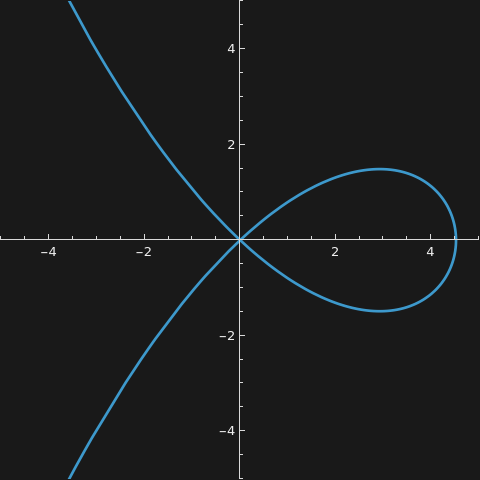
\includegraphics[width=0.5\linewidth]{trayectoria}
			\label{fig:trayectoria}
		\end{figure}
		
	\end{enumerate}
\end{enumerate}

\end{document}